%\section{Porous medium}

Soil or rock can be considered as a multiphase medium consisting
of a solid phase (solid matrix) and of one or more fluid phases
(gas and liquids), which occupy the void space (Fig.
\ref{fig:porous_medium}). Fluids are immiscible\index{fluid -
immiscible}, if a sharp interface is maintained between them. In
general, a phase is defined as a part of a continuum, which is
characterized by distinct material properties and by a
well-defined set of thermodynamic state variables. State variables
describe the physical behaviour at all points of the phase. They
must vary continuously within the considered phase of a continuum.
Phases are separated from each other by surfaces referred to as
interphase boundaries. Transport of components may occur within a
phase and/or across interphase boundaries. Those
interphasic\index{process - interphase} exchange processes between
adjacent phases can result from diffusive and/or advective
mechanisms.

In fact, it is impossible to describe the complex geometry of the
solid matrix and the topology of the void space at the microscopic
level, i.e. the topology of the pore space will never be known in
detail. As a consequence, boundary conditions for a mathematical
model cannot be stated at this scale, since they are not known at
the microscopic level. Moreover, it will be extremely difficult to
measure values of state variables at each point within a phase in
order to observe processes, to calibrate and to verify any model.
Finally, the complete formulation and resolution of balance
equations at the microscopic\index{scale - microscopic} level is
impossible and may not be reasonable. Therefore, it is necessary
to transform the problem from a microscopic scale to a
macroscopic\index{scale - macroscopic} level. Starting from the
microscopic balance equations for extensive quantities (masses,
momentum, energy), this procedure is the subject of the theory of
the porous medium 
\cite{Bea:72,Die:85,Ehl:89,BeaBac:90,Kin:1992,Hel:97,LewSch:98,Boe:00}
%(Bear 1972, Diersch 1985, Bear \& Bachmat 1990, de Boer \& Ehlers 1986, Lewis \& Schrefler 1998, de Boer 2000).
The entire problem is rewritten in terms of averages of
microscopic quantities, which have measurable values. The
resulting macroscopic model is referred to as the continuum
approach\index{model - continuum}. This conceptual model implies
that a real system is replaced by a number of overlapping continua
representing the corresponding phases. It is assumed that each
phase, occupying a certain part of the porous domain, is regarded
as a continuum. These individual phases interact with each other
at any place within the entire domain, because they are present at
each point within the porous medium, i.e. all phases are
completely mixed.
%
\begin{eqnarray}
\Omega_0
=
\sum_{\alpha} \Omega^\alpha
\end{eqnarray}
%
In addition to the porous medium approach, there exist different
types of structural models for fractured rocks, which characterize
the degree of inhomogeneity: the fractured medium\index{medium -
fractured} and the fractured porous medium\index{medium - porous
fractured}. The term fractured medium means that only the
fractures are important for the considered process, so blocks
surrounded by the fractures may be neglected in the model. The
term fractured porous medium means that both fracture system and
porous matrix are significant for the considered process. The
domain of a fractured porous medium consists of two subdomains,
representing heterogeneities at different scales, i.e. the
diameter of pores in the matrix and the characteristic length of
fractures.

Appropriate averaging rules must be defined in order to realize
the above described transformation from a microscopic to a
macroscopic level. For this purpose, a well-defined sample size of
an averaging volume must be found, which is referred to as the
representative elementary volume\index{volume - representative
elementary} (abbreviated REV). On the one hand, this averaging
unit has to be sufficiently large, so that the influence of
microscopic inhomogeneity on the values of averaged (macroscopic)
quantities will vanish, i.e. they become independent of size,
shape, and orientation of the REV. On the other hand, the REV must
be small enough to reflect the macroscopic heterogeneity. In
particular, the REV must be much smaller than the domain of
interest, which may vary in size for a flow or a transport
problem, respectively. From the mathematical point of view, the
macroscopic (averaged) quantities must be continuous and
differentiable functions (in space and in time), so that solutions
of the governing differential balance equations can be determined.
Finally, the continuum approach cannot be employed unless a common
range of a REV can be selected for all material properties (e.g.
porosity, permeability, dispersivity) as well as for all relevant
state variables. This requirement is important with respect to the
different conceptual models for fractured rock, which are
introduced in the following.

%=7.2==============================================================================
\subsection{Macroscopic Equations}

%\subsubsection*{Statistic approach}
%\index{model - statistic}

In fact, it is impossible to describe the complex geometry of the solid matrix
and the topology of the void space at the microscopic level, i.e. the topology
of the pore space will never be known in detail. Therefore, a statistical
approach is used for the derivation of balance equations at a macroscopic
level. The physical property of a porous medium is decomposed in phase-related
mean values $\overline{\psi^\alpha}$ and local fluctuations ${\psi'}^\alpha$.
%
\begin{eqnarray}
\psi^\alpha
=
\overline{\psi^\alpha}
+
{\psi'}^\alpha
\end{eqnarray}

%\subsubsection*{Averaging volume}
%\index{scale - averaging - volume}

An appropriate averaging volume is called
the Representative Elementary Volume (REV) (Fig. \ref{rev}).

% *** EPS-Grafik ***
\begin{figure}[htb!]
\begin{center}
\footnotesize
%\psfrag{Synonym}[pos][pos]{Tex-Ersetzung}
%\psfrag{x}[][]{$t$}
%\psfrag{y}[b][t]{$y(t)$}
%\psfrag{t}[][]{ }
%\includegraphics[height=7.5cm,width=11cm]{../figures/fig_71.bmp}
\includegraphics[width=0.95\columnwidth]{figures/por2.eps}  % Filename.eps
\caption{Definition of the representative elementary volume (REV) \cite{BeaBac:90}} 
\label{rev}
\end{center}
\end{figure}
%

%\subsubsection*{Averaging operator}

Several averaging procedures can be defined \cite{BeaBac:90}. As
an example we consider volumetric averaging which is also denoted as the
concept of volume fractions. The volumetric averaging operator is given by
%
\begin{eqnarray}
\overline{\psi^\alpha}^\alpha
=
\frac{1}{\epsilon^\alpha \Omega_0}
\int\limits_{\Omega_0} f^\alpha \psi^\alpha d\Omega
\label{eqn:mean}
\end{eqnarray}

where $\alpha$ is the phase indicator, $\epsilon^\alpha =
\Omega^\alpha/\Omega_0$ is the volumetric fraction of the $\alpha$
phase, $\Omega_0$ is the averaging volume (corresponding to the
representative elementary volume), $f^\alpha=1/0$ (inside or
outside $\alpha$ phase) is the phase distribution function.

%\subsubsection*{Averaging rules}
%\index{scale - averaging - rules}

Due to the above definition the following averaging rules can be derived.

\begin{itemize}
 \item Sum
\begin{eqnarray}
\overline{\psi_1^\alpha+\psi_2^\alpha}
=
\overline{\psi_1^\alpha}+\overline{\psi_2^\alpha}
\end{eqnarray}

 \item Product
\begin{eqnarray}
\overline{\psi_1^\alpha \psi_2^\alpha}
=
\overline{\psi_1^\alpha}\,\overline{\psi_2^\alpha}
+
\overline{{\psi_1'}^\alpha {\psi_2'}^\alpha}
\end{eqnarray}

 \item Time derivative
\begin{eqnarray}
\epsilon^\alpha \overline{\frac{\partial \psi^\alpha}{\partial t}}
=
\frac{\partial \epsilon^\alpha \overline{\psi^\alpha}}{\partial t}
-
\frac{1}{\Omega_0}
\int\limits_{S^{\alpha\beta}}\psi^\alpha {\bf w} \cdot d{\bf S}
\end{eqnarray}

 \item Spatial derivative
\begin{eqnarray}
\epsilon^\alpha \overline{\nabla\psi^\alpha}
=
\nabla(\epsilon^\alpha\overline{\psi^\alpha})
+
\frac{1}{\Omega_0}
\int\limits_{S^{\alpha\beta}}\psi^\alpha \cdot d{\bf S}
\end{eqnarray}

\end{itemize}

where $\bf w$ is the velocity of the $\alpha\beta$-phase interface.

%\subsubsection*{General macroscopic balance equation}
%\index{equation - general balance}

To derive a phase related macroscopic balance equation,
we have to average the balance equation in differential form
for a certain phase (\ref{eqn:general_balance_equation}).
By use of the above averaging operators and rules
the following general macroscopic balance equation
can be obtained.
%
\begin{eqnarray}
\frac{\partial \epsilon^\alpha \overline{\psi^\alpha}}{\partial t}
=
-
\nabla\cdot(
\epsilon^\alpha\bar{\psi^\alpha}\overline{{\bf v}^\alpha}
+
\epsilon^\alpha\overline{{\psi'}^\alpha{\bf v'}^\alpha}
+
\epsilon^\alpha\overline{{\bf\Phi}_{\textrm{\tiny Diff}}^{\psi^\alpha}}
)
\nonumber \\
-
\frac{1}{\Omega_0}
\int\limits_{S^{\alpha\beta}} {\bf\Phi}_{\textrm{\tiny Diff}}^{\psi^\alpha} \cdot d{\bf S}
-
\frac{1}{\Omega_0}
\int\limits_{S^{\alpha\beta}}\psi^\alpha ({\bf v-w}) \cdot d{\bf S}
+
q^{\psi^\alpha}
\end{eqnarray}

with the dispersive flux
\begin{eqnarray}
{\bf\Phi}_{\textrm{\tiny Disp}}^{\psi^\alpha}
=
\epsilon^\alpha\overline{{\psi'}^\alpha{\bf v'}^\alpha}
\end{eqnarray}

%------------------------------
\subsection{Theory of Mixtures}
\label{sec:mixtures}

The Theory of Mixtures as one of the basic approaches to model the complex behavior of porous media has been developed over decades (concerning basic assumptions see e.g. \cite{Bow:1976,TT:1960}). As the Theory of Mixtures does not incorporate any information about the microscopic structure of the material\footnote{Within the context of the Theory of Mixtures the ideal mixture of all constituents of a multiphase medium is postulated. Consequently, the realistic modeling of the mutual interactions of the constituents is difficult.}, it has been combined with the Concept of Volume Fractions by e.g. \cite{Bow:1980,BE:1986a,LewSch:98,Pre:1980}. Within the context of this enhanced Theory of Mixtures (also known as Theory of Porous Media), all kinematical and physical quantities can be considered at the macroscale as local statistical averages of their values at the underlying microscale.
%
Concerning a detailed overview about the history of the modeling of the behavior of multiphase multicomponent porous media, the reader is referred to e.g. \cite{Boe:00}. Comprehensive studies about the theoretical foundation and numerical algorithms for the simulation of coupled problems of multiphase continua are given in e.g. \cite{Boe:00,EB:2002,LewSch:98} and the quotations therein. 

The individual constituents $\varphi^{\alpha}$ of a porous material represent the phases of the overall aggregate or components within a phase. Below, $\alpha=s$ marks one immiscible solid phase (no sorption processes are considered), and $\alpha=\gamma$ denote several immiscible pore fluid phases. 
%
A porous medium, however, consists of multiple phases (fluids such as water, air and non-aqueous phase liquids (NAPLs) as well as solids). 
Moreover, these phases can contain several chemical components which can be dissolved in liquids or adsorbed to the solid phase (Fig. \ref{fig:porous_medium}).

\newpage
.
\vspace{4cm}
\begin{figure}[htbp]
\hspace{3cm}
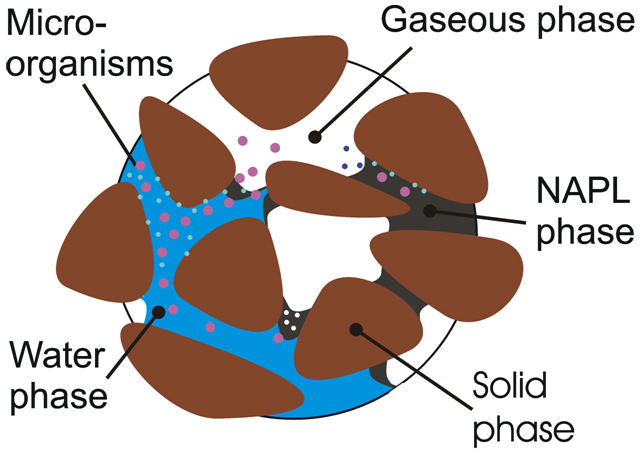
\includegraphics[width=0.06\columnwidth]{figures/pm}
\caption{Conceptual approach of a porous medium model, adopted from \cite{Kol:02}}
\label{fig:porous_medium}
\end{figure}

Within the framework of the Concept of Volume Fractions, scalar variables like volume fractions and saturations are defined to describe the microstructure of a porous medium in a macroscopic manner neglecting the real topology and distribution of the pores. These variables serve as measures of local fractions of the individual constituents. The volume fractions $n^{\alpha}$ represent the ratio of the partial volume $dv^{\alpha}$ of a given constituent $\varphi^{\alpha}$ of a multiphase body with respect to the overall volume $dv$ of a representative elementary volume (REV) of the control domain $\Omega$ under consideration. Consequently, based on the definitions of the overall volume of the control domain
\begin{equation}
V=\int\limits_{\Omega}\,dv
\label{eq1}
\end{equation}
and the corresponding partial volumes of the individual constituents
\begin{equation}
V^{\alpha}=\int\limits_{\Omega}\,dv^{\alpha}\qquad\mbox{with}\qquad V=\sum\limits_{\alpha}\,V^{\alpha}
\label{eq2}
\end{equation}
the volume fractions
\begin{equation}
n^{\alpha}=\frac{dv^{\alpha}}{dv}
\label{eq3}
\end{equation}
provide some information about the local volume distribution of the individual constituents.
\begin{equation}
V^{\alpha}=\int\limits_{\Omega}\,dv^{\alpha}=\int\limits_{\Omega}\,n^{\alpha}\,dv
\label{eq4}
\end{equation}
One of the most characteristic media properties of a porous material is the porosity, the local amount of fluid volume fractions.
\begin{equation}
n=\sum\limits_{\gamma}\,n^{\gamma}=1\,-\,n^s
\label{eq5}
\end{equation}
Since, in general, the overall medium is completely filled with matter, from Eqn.~(\ref{eq2}) follows the saturation condition regarding the overall aggregate.
\begin{equation}
\sum\limits_{\alpha}\,n^{\alpha}=1
\label{eq6}
\end{equation}

If multiphase flow occurs, it is more convenient for various applications to use the (partial) fluid saturations $S^{\gamma}$ instead of the volume fractions. These local functions are given by
\begin{equation}
S^{\gamma}=\frac{dv^{\gamma}}{dv-dv^s}=\frac{n^{\gamma}}{n}
\label{eq7}
\end{equation}
obviously fulfilling the saturation condition regarding the pore content.
\begin{equation}
\sum\limits_{\gamma}\,S^{\gamma}=1
\label{eq8}
\end{equation}

Usually, constraint conditions addressing real physical effects are formulated to simplify complex mathematical and numerical models. Within the context of porous media, it is reasonable in most applications to assume the (material) incompressibility of constituents as a substantial constraint condition. The issue of (in)compressibility of a material is closely connected to the possible temporal evolution of its mass density.

Within the framework of the Concept of Volume Fractions, two different formulations of mass density related to the constituents of a porous medium are introduced. The so-called material (effective, realistic) density $\rho^{\alpha R}$ is defined as the ratio of the mass fraction $dm^{\alpha}$ of the given individual constituent $\varphi^{\alpha}$ with respect to its partial volume fraction.
\begin{equation}
\rho^{\alpha R}=\frac{dm^{\alpha}}{dv^{\alpha}}
\label{eq9}
\end{equation}
In contrast, the so-called partial (global, bulk) density is given by the ratio of the mass fraction of the constituent under consideration with respect to the volume fraction of the overall aggregate.
\begin{equation}
\rho^{\alpha}=\frac{dm^{\alpha}}{dv}
\label{eq10}
\end{equation}
Based on the definition of the volume fractions (\ref{eq3}), the material and the partial densities are correlated to each other.
\begin{equation}
\rho^{\alpha}=n^{\alpha}\,\rho^{\alpha R}
\label{eq11}
\end{equation}
If the volume fractions change with time under external loading, from Eqn.~(\ref{eq11}) follows that for an intrinsically incompressible individual constituent (constant material mass density) compressibility referred to the overall aggregate is observed.
\begin{equation}
\rho^{\alpha R}=\mbox{const} \quad\Rightarrow\quad
\rho^{\alpha}\,\neq\,\mbox{const}\quad\mbox{as}\quad n^{\alpha}\,\neq\,\mbox{const}
\label{eq12}
\end{equation}

Obviously, the mass density of the porous medium (homogenized overall aggregate) is defined as the sum of the partial densities of its constituents.
\begin{equation}
\rho=\sum\limits_{\alpha}\rho^{\alpha}
\label{eq13}
\end{equation}

The conceptual idea behind the formulations and relations presented above consists in the assumption that the mass fractions of all constituents of the multiphase medium are simultaneously present and statistically uniformly distributed over the entire control domain. Within this context, the material body under consideration is theoretically substituted by an aggregate completely and continuously filled by superimposed (overlapping) homogenized partial continua. In other words, all constituents of a porous medium are characterized as smeared substitute continua with reduced mass densities. Consequently, the motion and physics of the individual constituents as well as the overall aggregate can be specified by well-accepted phenomenological methods of continuum mechanics.

Describing the transport and deformation of the constituents of porous media within the framework of continuum mechanics it is assumed that the geometry of the control domain under consideration is characterized at each time by the solid skeleton, whereas the fluid pore content is able to flow across the boundary of the surface. This assumption serves as conceptual nucleus for the simulation of complex, coupled physical processes in multiphase porous media, particularly if a deformable solid skeleton is observed. Within this context, it proves to be reasonable not to model the absolute motion state of the pore content, but its motion relative to the motion of the solid phase, considering the porous medium as a local thermodynamic open system with the solid skeleton as volume under observation.

The macroscopic characterization of the physical processes considering the real microstructural situation in a statistically averaged manner is completely adequate for the most hydrological, geotechnological and biomechanical problems under consideration (cf. \cite{GWASG:2006} and others).